\documentclass[7pt,a4paper]{article}

\usepackage{graphicx}
\usepackage{sectsty}

\sectionfont{\fontsize{10}{11}\selectfont}
\subsectionfont{\fontsize{10}{11}\selectfont}

\begin{document}
\textbf{\LARGE Assignment 2a Report - Text Mining}
\section{Introduction}
Given a collection of text documents we aim to find similar documents. In order to do that we normalized the text and created a similarity matrix using Jaccard Index. Also applied hierarchical clustering in order to identify clusters of similar documents.

\section{Packages Used - \textit{(Language: Python)}}
\begin{itemize}
\item{\textbf{NLTK}: Package used for Natural Language Processing.}
\item{\textbf{Scipy}: Package which provides function for plotting dendogram and linkage for Hierarchical Clustering.}
\item{\textbf{Seaborn}: Used for visualization of data through plots}
\item{\textbf{Matplotlib}: Used for plotting of graphs}
\item{\textbf{Pandas}: Package which provides Data structure like DataFrame which makes
manipulation of datasets easy}
\end{itemize}

\section{Dataset}
Twenty two text documents were taken all being on the Topic- \textbf{‘The History of web search engines’}.

\section{Pre-Processing of Text Documents}
\begin{enumerate}
\item{\textit{Tokenizing} text into sentences and then into words called tokens}
\item{\textit{Case Folding} - All words were converted to lower case}
\item{Removing punctuations and digits}
\item{Removing stopwords - \textit{(Used Standard stop words list for English language)}}
\begin{itemize}
\item{Stops word list were customized according to the domain by adding \textit{search}, \textit{engine} to the list}
\end{itemize}
\item{Performing stemming \textit{(Porter Stemmer)}}
\end{enumerate}

\section{Methods}
\subsection{Jaccard Coefficient}
\begin{itemize}
\item{Used to calculate similarity between two sets A and B
$$ J.C. = \frac{n(A \cap B)}{n(A \cup B)} $$}
\item{Value varies between 0 and 1 where 0 indicates \textit{no similarity} and 1 indicates \textit{complete similarity}}
\item{\textbf{Similarity matrix} is obtained as shown in the figure \ref{image-J-C} by calculating jaccard coefficient between each pair of documents}
\end{itemize}
\begin{figure}[h]
\centering
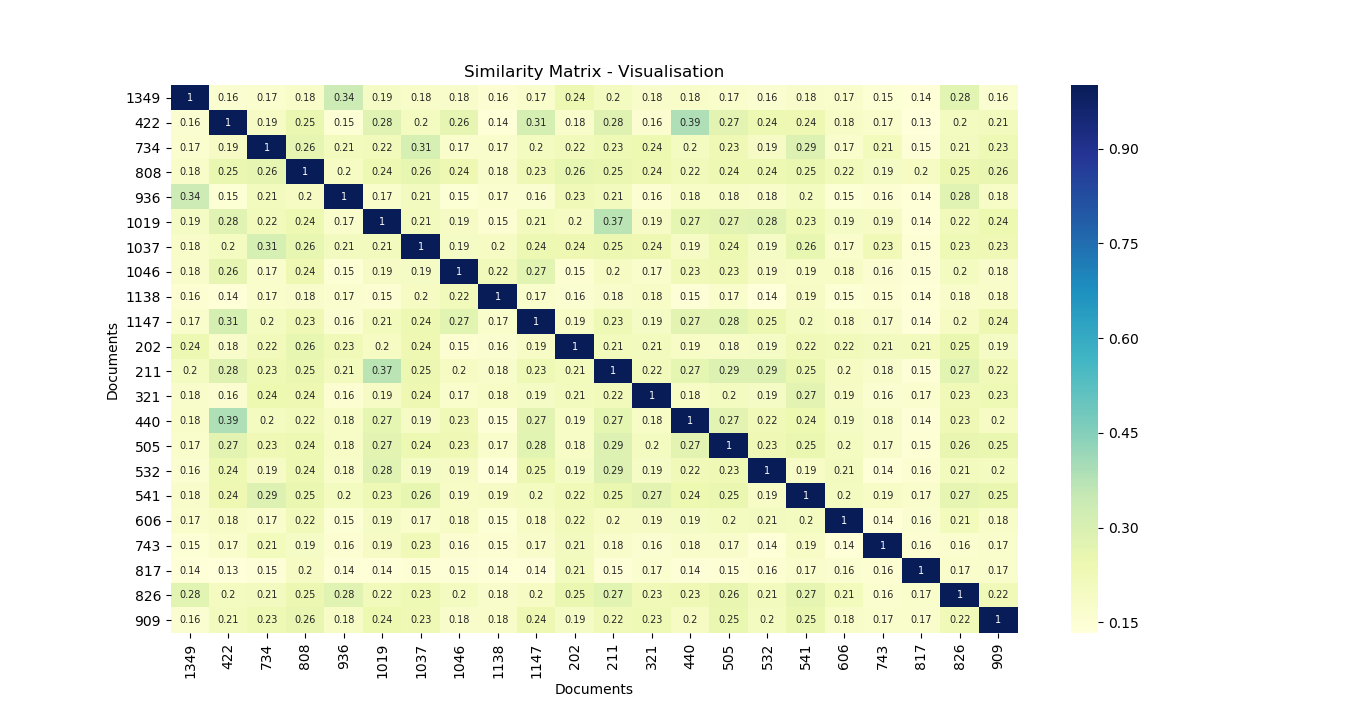
\includegraphics[scale=.40]{Heatmap}
\caption{Similarity matrix - Jaccard Cofficient}
\label{image-J-C}
\end{figure}


\subsection{Hierarchical Clustering}
\begin{itemize}
\item{\textbf{Distance matrix}: It is obtained by calculating \textit{(1-Jaccard Coefficient)} between each pair of the documents}
\item{\textbf{Linkage Parameter} : Single Linkage}
\item{Dendogram is shown in the figure \ref{image-Dendogram} below where the horizontal axis represents the pairwise dissimilarity between documents}
\end{itemize}

\section{Observations}
\subsection{Jaccard Coefficient}
\begin{itemize}
\item{It does not normalize the lengths of the documents so smaller documents has higher similarity as compared to larger documents in case the cardinality of the set of common words is almost similar.}
\begin{itemize}
\item{For instance, The documents \textit{Ass1-211} (Length - 359) \& \textit{Ass1-826} (Length - 240) has 100 words and 105 words in intersection with the document \textit{Ass1-1349} respectively which is almost same but due to the difference in the length of the documents the first one has 0.198 similarity while the latter one has 0.275 similarity with the document}
\end{itemize}
\item{According to the similarity matrix, most similar documents comes out to be \textit{Ass1-422} and \textit{Ass1-440} (Similarity - 0.39) while the most dissimilar documents are \textit{Ass1-817} and \textit{Ass1-422} (Similarity - 0.1336)}
\end{itemize}

\subsection{Hierarchical Clustering}
\begin{figure}[h]
\centering
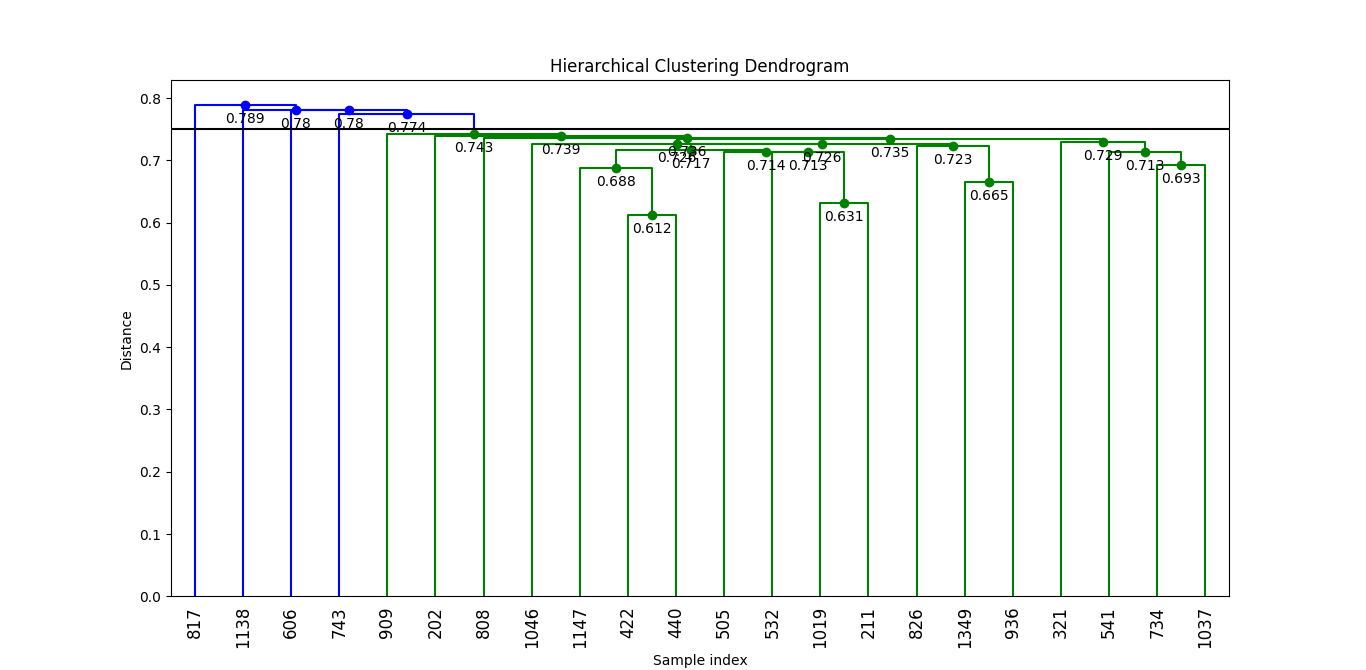
\includegraphics[scale=.35]{dendro}
\caption{Dendogram - Hierarchical Clustering}
\label{image-Dendogram}
\end{figure}

\begin{itemize}
\item{\textbf{Elbow Method} (Determining number of clusters)- Maximum acceleration of distance growth in the curve as shown in the figure \ref{image-elbow-method} is obtained from 5 to 6. Hence, Elbow Method suggests that number of clusters would be five. This is also verified with the help of dendrogram where the cut is obtained at the highest jump of distance.}
\item{As observed through the Dendrogram cut at d = 0.75, we have obtained \textit{five clusters} out of the collection of documents}
\item{Documents \textit{Ass1-422} and \textit{Ass1-440} comes out to be most similar (Distance - 0.612)}
\item{Documents \textit{Ass1-817} is most dissimilar to all other documents}
\end{itemize}

\begin{figure}[h]
\centering
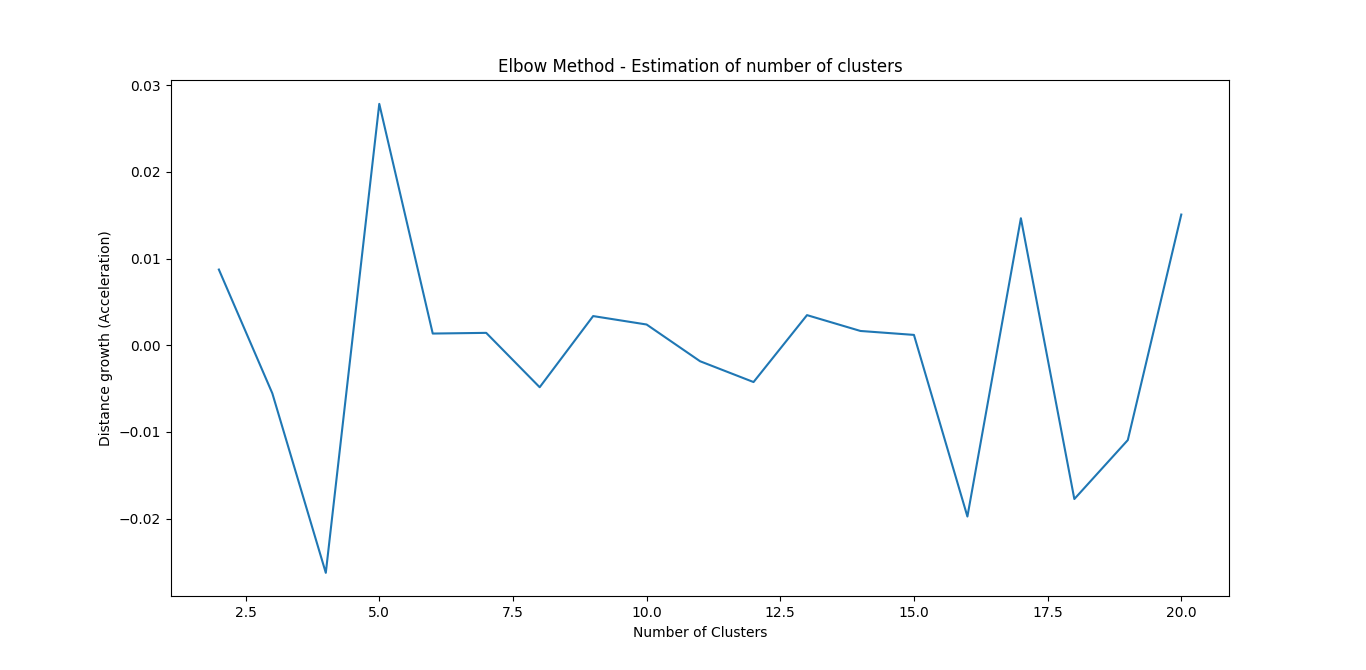
\includegraphics[scale=.30]{elbow}
\caption{Curve obtained - Elbow method}
\label{image-elbow-method}
\end{figure}


\end{document}
